\subsection{Numerical results}
\label{sec:complement-results}
Pointwise deviations from theory quoted below use
$100[\delta_{a\mid b}(y)/F_{\rm CFT}(y)-1]$ percent, with the
theoretical value in the denominator.
The computation completes all fifteen sizes through $N=256$ for both
CFTs, with $\ell=4,\ldots,12$. All deficits are positive. The original
checks and extension checks are reported in Tables~\ref{tab:complement-checks}
and \ref{tab:complement-extension-checks}. The narrower window changes
only the selected observations and fitted parameters; all previous
relative-entropy values are preserved.

For Ising $I\mid\sigma$ and $\sigma\mid I$, the free exponents are
$0.2853$ and $0.2853$,
compared with $1/4$, with coefficients
$0.57468$ and $0.57465$,
compared with $B_{ab}=0.46544$.
For $I\mid\varepsilon$ and $\varepsilon\mid I$, the exponents are
$1.9691$ and $2.0140$,
compared with $2$. For $\sigma\mid\varepsilon$ and $\varepsilon\mid\sigma$,
they are $0.2376$ and
$0.3298$, compared with $1/4$.
Their deficit-to-leading ratios at $N=256,\ell=12$ are
$0.9827$ and
$1.1567$, respectively.
This endpoint is outside the fitting window.

For boson $00\mid ss$ and $ss\mid00$, the free exponents are
$0.9757$ and $0.9748$,
compared with $1$. For $00\mid3s,s$ and its reverse, they are
$4.8120$ and $4.8243$,
compared with $5$, with fitted coefficients
$0.12188$ and $0.12456$,
compared with $5\pi/64\simeq0.24544$.
For $ss\mid3s,s$ and its reverse, the exponents are
$1.9532$ and $1.9559$,
compared with $2$.

These are effective powers over $y\leq0.04$. The coefficient and
exponent are correlated, so a small residual alone does not establish
the analytical asymptote. Tables~\ref{tab:ising-complement-fits} and
\ref{tab:boson-complement-fits} separately compare the free fit and the
amplitude fit with imposed analytical exponent. The added $\ell=11,12$
points test their continuation outside this window; they do not change
the fitted coefficients. Increasing $N$ at fixed $\ell$ makes $y$ smaller
without increasing the number of sites in $A$. The displayed discrepancies
do not by themselves distinguish omitted continuum terms from finite
lattice effects. No lattice-correction fitting formula is introduced.

Figures~\ref{fig:ising-complement-entropy}--\ref{fig:boson-complement-residuals}
show all twelve directed comparisons. Each row contains the two
directions of one mixture. The gray region is displayed but excluded
from fitting. Tables~\ref{tab:ising-complement-fits} and
\ref{tab:boson-complement-fits} separately report the free
coefficient/exponent fit, the amplitude fit with the analytical exponent
fixed, and the analytical CFT leading-order prediction with no fitted
parameters, including residual and
cross-validation measures.
Table~\ref{tab:complement-endpoint} gives the $N=256$ endpoint values
and ratios to the analytical leading term at $\ell=4,12$.

\begin{figure}[p]
\centering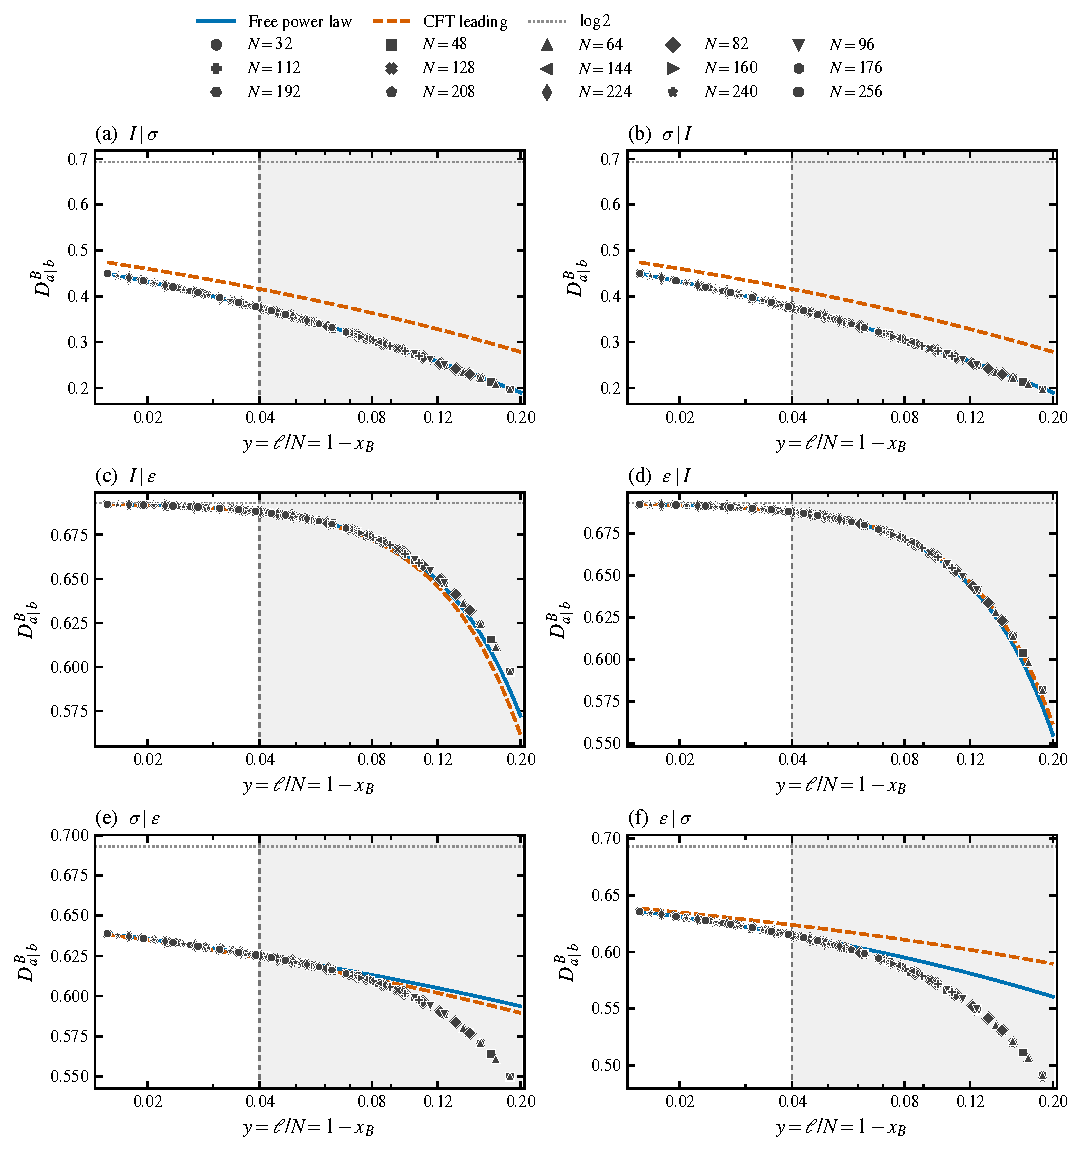
\includegraphics[width=.97\textwidth]{../figs/ising_complement_entropy.pdf}
\caption{Ising large-interval mixture relative entropies
$D^B_{a\mid b}=S(\rho_a^B\|(\rho_a^B+\rho_b^B)/2)$, with $p=1/2$.
The source and other primary are indicated as $a\mid b$ in each panel.
$A$ has $\ell=4,\ldots,12$ sites and $B$ has $N-\ell$ sites;
$N=32,48,64,82,96,112,128,144,160,176,192,208,224,240,256$.
All 126 points per direction at $y=\ell/N\leq0.20$ are shown.
Only the 39 points at $y\leq0.04$ enter the free fit
$D_B=\log2-\widehat C(\pi y)^{\widehat\beta}$; both parameters vary.
The dashed curve is the analytical CFT leading-order prediction
$\log2-B_{ab}(\pi y)^{\beta_{\rm CFT}}$, with both parameters from
Table~\ref{tab:complement-theory} and no fitting; the dotted line is $\log2$.
The gray region is excluded from fitting. Natural logarithms, exact
Jordan--Wigner primaries, and Gram threshold $10^{-15}$ are used.
The support reduction uses cutoff $10^{-16}$, with full $N=256$ references (Sec.~\ref{sec:complement-extension-checks}). Fit parameters are in Table~\ref{tab:ising-complement-fits}.}
\label{fig:ising-complement-entropy}
\end{figure}
\begin{figure}[p]
\centering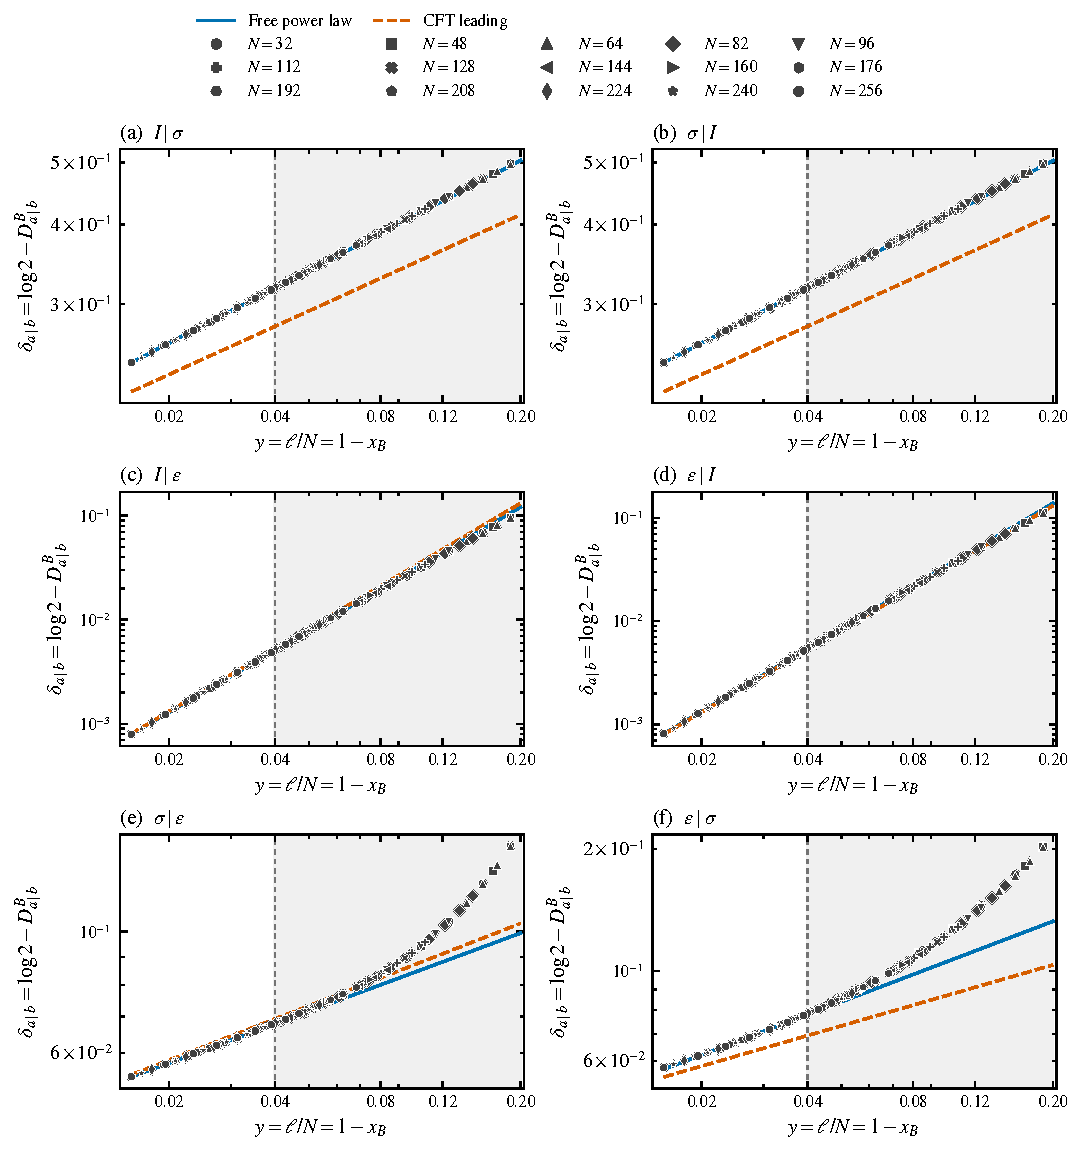
\includegraphics[width=.97\textwidth]{../figs/ising_complement_deficit.pdf}
\caption{Ising deficits $\delta_{a\mid b}=\log2-D^B_{a\mid b}$ for
$p=1/2$, $N=32,48,64,82,96,112,128,144,160,176,192,208,224,240,256$
and $\ell=4,\ldots,12$. There are 126 displayed samples per direction
at $y\leq0.20$ and 39 fitted samples at $y\leq0.04$.
Both axes are logarithmic. The free fit is
$F(y)=\widehat C(\pi y)^{\widehat\beta}$; the dashed curve is the
analytical CFT leading-order prediction $B_{ab}(\pi y)^{\beta_{\rm CFT}}$,
with no fitted parameters. The two analytical powers are
$\beta_{\rm CFT}=1/4$ for the spin channels and $2$ for
$I,\varepsilon$, with coefficients in Table~\ref{tab:complement-theory}.
The gray region is excluded from fitting.
Natural logarithms and Gram threshold $10^{-15}$ are used.
The support reduction uses cutoff $10^{-16}$, with full $N=256$ references (Sec.~\ref{sec:complement-extension-checks}). Table~\ref{tab:ising-complement-fits} reports both fitted parameters.}
\label{fig:ising-complement-deficit}
\end{figure}
\begin{figure}[p]
\centering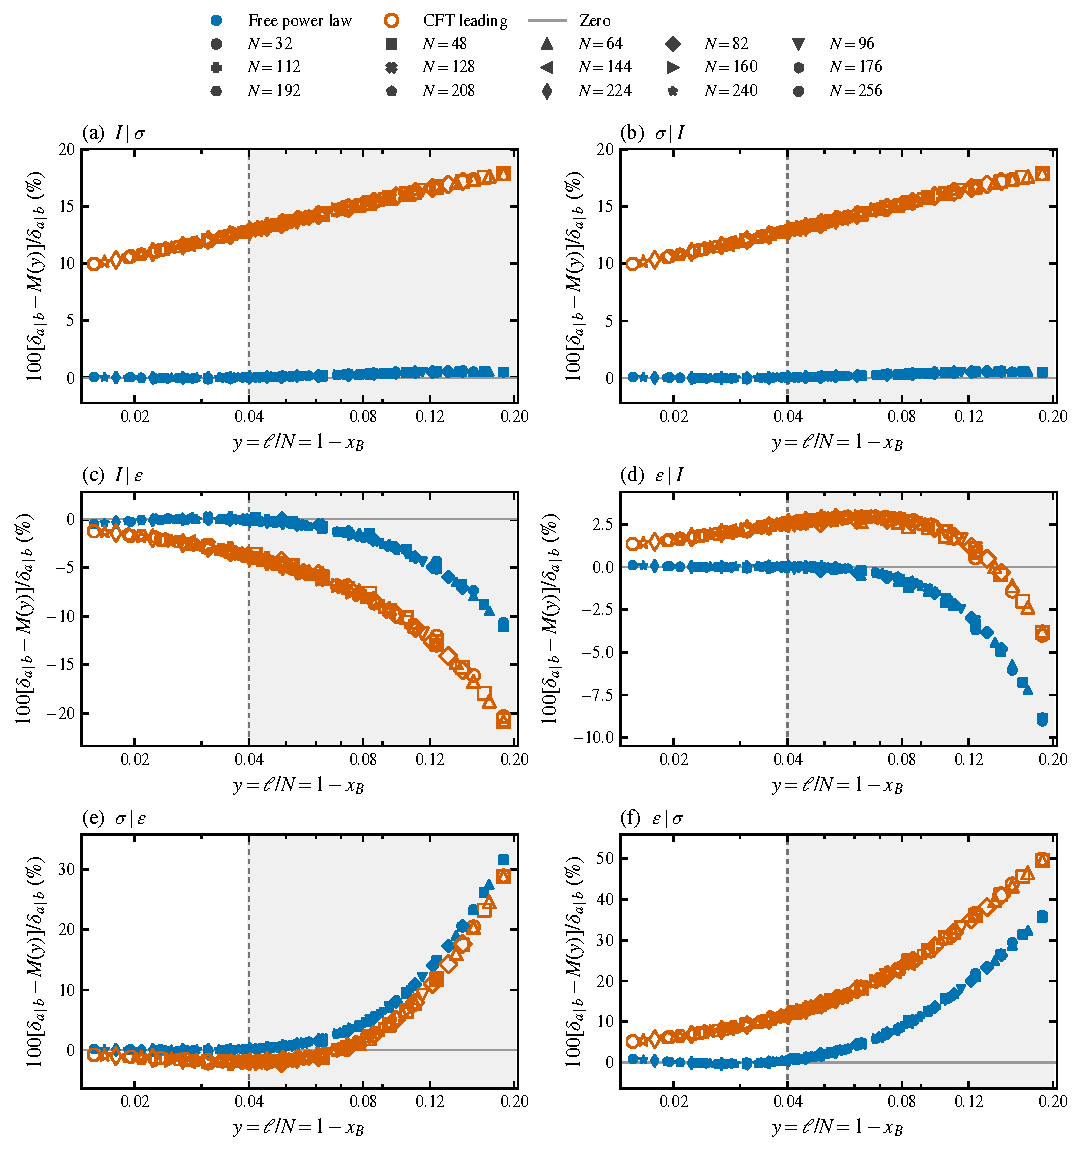
\includegraphics[width=.97\textwidth]{../figs/ising_complement_residuals.pdf}
\caption{Ising relative deficit residuals
$R_i=100[\delta_i-M(y_i)]/\delta_i$ for $p=1/2$,
$N=32,48,64,82,96,112,128,144,160,176,192,208,224,240,256$,
$\ell=4,\ldots,12$. Blue markers show residuals of the free power-law fit
$M=\widehat C(\pi y)^{\widehat\beta}$. Orange markers show residuals of
the analytical CFT leading-order prediction
$M=B_{ab}(\pi y)^{\beta_{\rm CFT}}$, with both coefficient and exponent
from Table~\ref{tab:complement-theory} and no fitted parameters.
There are 126 displayed samples at $y\leq0.20$; 39 with $y\leq0.04$
determine the fit. The gray region is excluded from fitting.
The vertical scale is linear throughout and its ticks show $R_i$ in percent.
The horizontal $y$ axis is logarithmic. Natural logarithms and Gram threshold $10^{-15}$
apply; the support reduction uses cutoff $10^{-16}$, with full $N=256$ references (Sec.~\ref{sec:complement-extension-checks}). Table~\ref{tab:ising-complement-fits} gives the parameters,
RMSE and size-based CV RMSE defined in
Eqs.~\eqref{eq:complement-fit-metrics} and \eqref{eq:complement-cv}.}
\label{fig:ising-complement-residuals}
\end{figure}
\begin{figure}[p]
\centering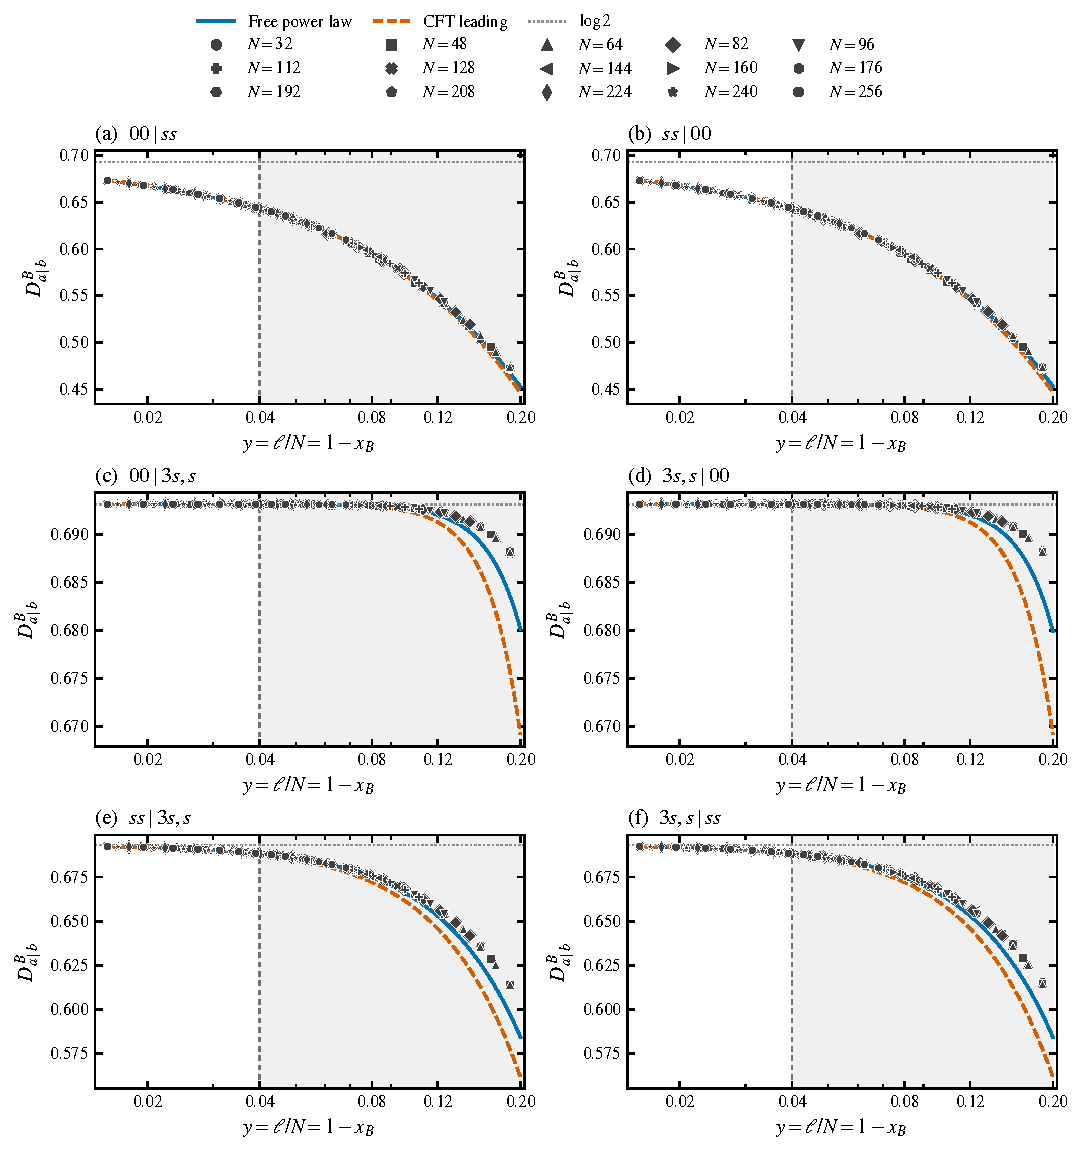
\includegraphics[width=.97\textwidth]{../figs/boson_complement_entropy.pdf}
\caption{Compact-boson large-interval relative entropies
$D^B_{a\mid b}=S(\rho_a^B\|(\rho_a^B+\rho_b^B)/2)$ at $p=1/2$,
$s=1/\sqrt2$, endpoint $W=10^8$, and 100-digit Pfaffian contractions.
The grid is $N=32,48,64,82,96,112,128,144,160,176,192,208,224,240,256$,
$\ell=4,\ldots,12$, with $A$ of size $\ell$ and $B$ its complement.
All 126 points at $y=\ell/N\leq0.20$ are shown; the 39 at
$y\leq0.04$ enter the free fit $\log2-\widehat C(\pi y)^{\widehat\beta}$.
The dashed curve is the analytical CFT leading-order prediction
$\log2-B_{ab}(\pi y)^{\beta_{\rm CFT}}$, with both parameters from
Table~\ref{tab:complement-theory} and no fitting; the dotted line is $\log2$.
The gray region is excluded from fitting.
Natural logarithms and Gram threshold $10^{-15}$ are used.
The support reduction uses cutoff $10^{-16}$, with full $N=256$ references (Sec.~\ref{sec:complement-extension-checks}). Table~\ref{tab:boson-complement-fits} gives both fitted parameters.}
\label{fig:boson-complement-entropy}
\end{figure}
\begin{figure}[p]
\centering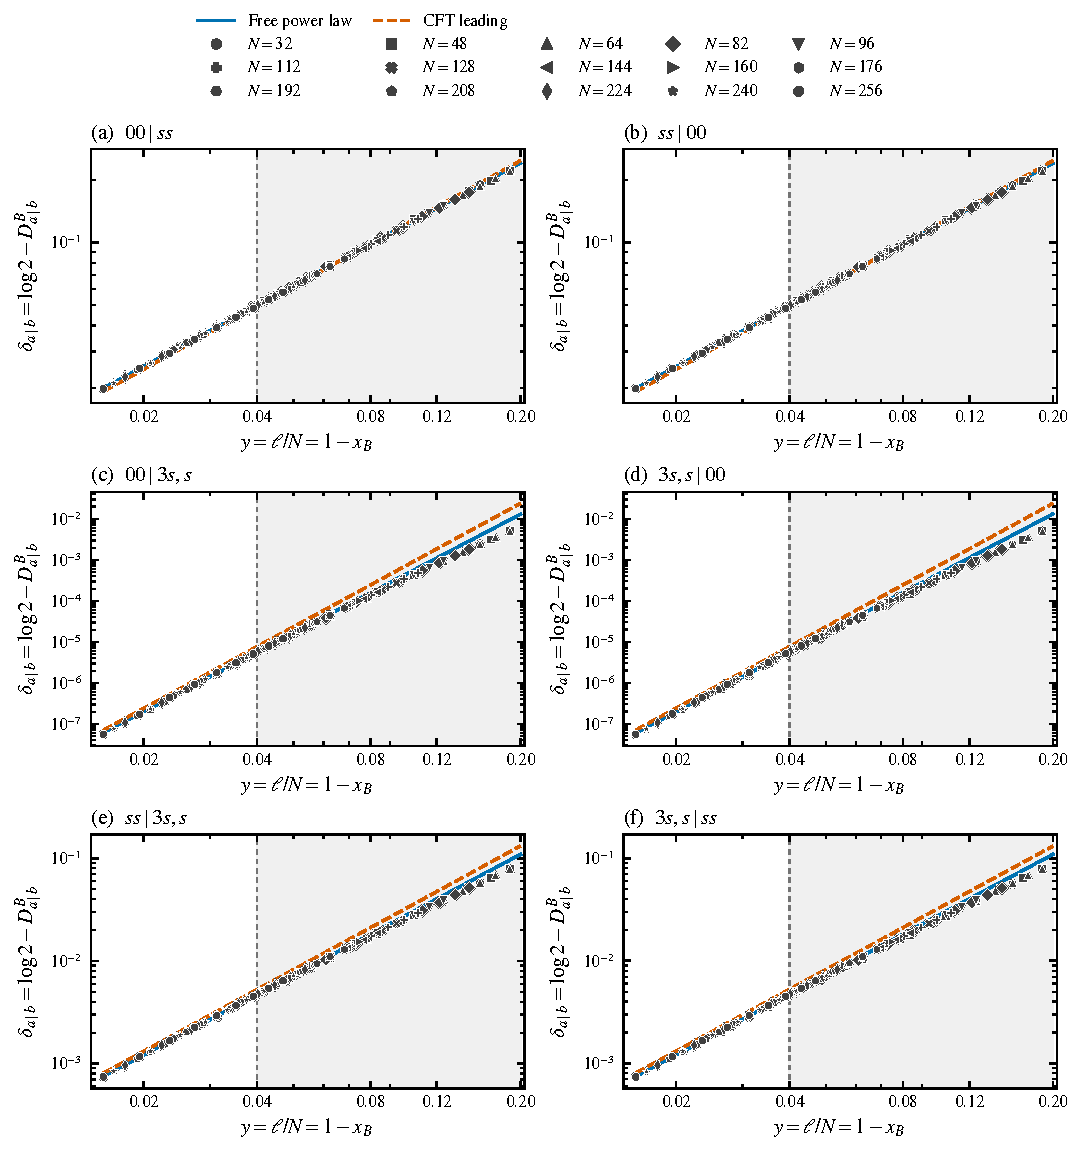
\includegraphics[width=.97\textwidth]{../figs/boson_complement_deficit.pdf}
\caption{Compact-boson deficits $\delta_{a\mid b}=\log2-D^B_{a\mid b}$
at $p=1/2$, $s=1/\sqrt2$, $W=10^8$, using 100-digit Pfaffians.
The grid is $N=32,48,64,82,96,112,128,144,160,176,192,208,224,240,256$,
$\ell=4,\ldots,12$; 126 samples at $y\leq0.20$ are displayed and 39
at $y\leq0.04$ enter the free fit.
The curves compare the free fit $F(y)=\widehat C(\pi y)^{\widehat\beta}$
with the analytical CFT leading-order prediction
$B_{ab}(\pi y)^{\beta_{\rm CFT}}$, with no fitted parameters. Its powers are
$1,5,2$ for $00,ss$; $00,3s,s$; and $ss,3s,s$, respectively.
Both axes are logarithmic; the gray region is excluded from fitting.
Natural logarithms and Gram threshold $10^{-15}$ are used.
The support reduction uses cutoff $10^{-16}$, with full $N=256$ references (Sec.~\ref{sec:complement-extension-checks}). Tables~\ref{tab:complement-theory} and \ref{tab:boson-complement-fits}
give the analytical and fitted parameters.}
\label{fig:boson-complement-deficit}
\end{figure}
\begin{figure}[p]
\centering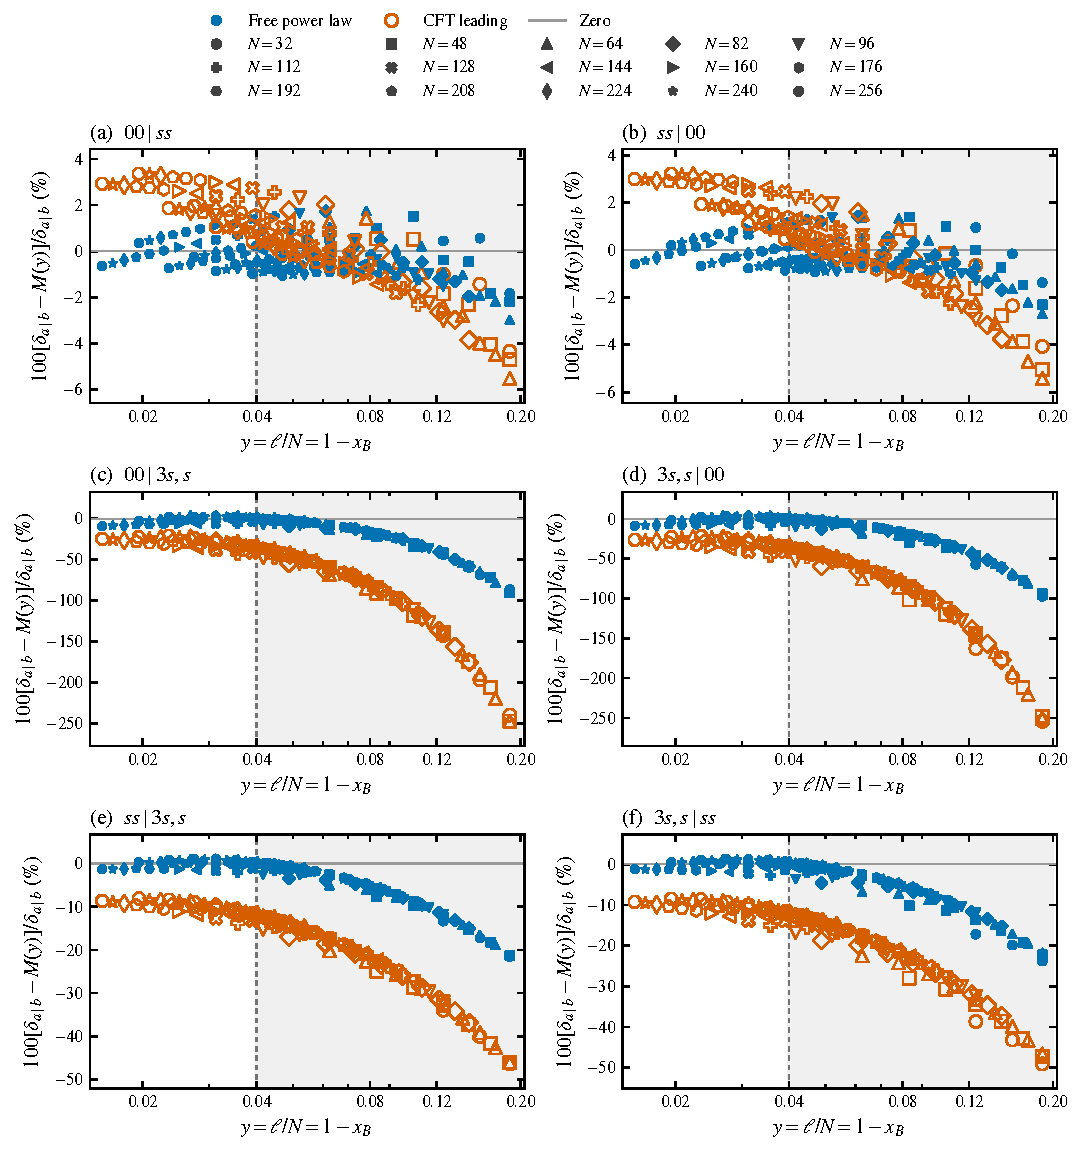
\includegraphics[width=.97\textwidth]{../figs/boson_complement_residuals.pdf}
\caption{Compact-boson residuals
$R_i=100[\delta_i-M(y_i)]/\delta_i$ at $p=1/2$, $s=1/\sqrt2$,
$W=10^8$, with 100-digit Pfaffians and Gram threshold $10^{-15}$.
The grid is $N=32,48,64,82,96,112,128,144,160,176,192,208,224,240,256$,
$\ell=4,\ldots,12$. Blue markers show residuals of the free power-law fit
$M=\widehat C(\pi y)^{\widehat\beta}$. Orange markers show residuals of
the analytical CFT leading-order prediction
$M=B_{ab}(\pi y)^{\beta_{\rm CFT}}$, with both coefficient and exponent
from Table~\ref{tab:complement-theory} and no fitted parameters.
All 126 samples at $y\leq0.20$ are displayed; the 39 at $y\leq0.04$
determine the free fit. The gray region is excluded from fitting.
The vertical scale is linear throughout and its ticks show $R_i$ in percent.
The horizontal $y$ axis is logarithmic. Natural logarithms apply. The support reduction uses cutoff $10^{-16}$, with full $N=256$ references (Sec.~\ref{sec:complement-extension-checks}).
Table~\ref{tab:boson-complement-fits} gives both parameter comparisons,
RMSE and size-based CV RMSE.}
\label{fig:boson-complement-residuals}
\end{figure}
\clearpage
